% !TEX root = report.tex

\chapter{Bot Architecture}

This chapter will describe the overall structure of \massexpand and provide descriptions of the major components.

\section{Overall Structure}

The starting point of the creation of the bot was the example AI module distributed with BWAPI. The example contains the main update loop of the bot, all event listeners BWAPI supports and methods for drawing extra information on the screen. It also provides some sample code for giving orders to units. We left the example module mostly intact, except for the units orders which we removed completely. We added calls to methods of a new class, HighCommand, which would be the control center for our code. The main benefits of this were that we kept the example code for reference, and that if there would be a major change in BWAPI, we could use the new example module and quickly plug in our own code.

In our first attempts to create a bot, we tried using BWSAL, a collection of classes forming an abstraction layer for BWAPI. These classes provide methods for common tasks such as assigning workers to collect resources, maintaining a build queue and finding suitable building places. We quickly abandoned BWSAL after realizing it would be hard to adapt it to our ideas. What we kept from BWSAL were two helper classes, UnitGroup (an excellent class to select and divide groups of units) and BuildingPlacer (a class with methods to determine where a building should be built). We also kept the overall structure BWSAL used, including the naming scheme (the "managers").

The managers are all responsible for a part of the performance of the bot. For example, we have a manager keeping track of our minerals and gas, a manager storing information about enemy units and a manager overseeing construction of buildings and units. Organizing the bot this way allows us to seperate code pertaining to different areas of the bot operation, and also allows us to structure the way the information obtained from the game flows through our bot, resulting in commands sent back to the game. This flow of information is shown in Figure~\ref{fig:flowofinformation}.

\begin{figure}[htb]
\centering
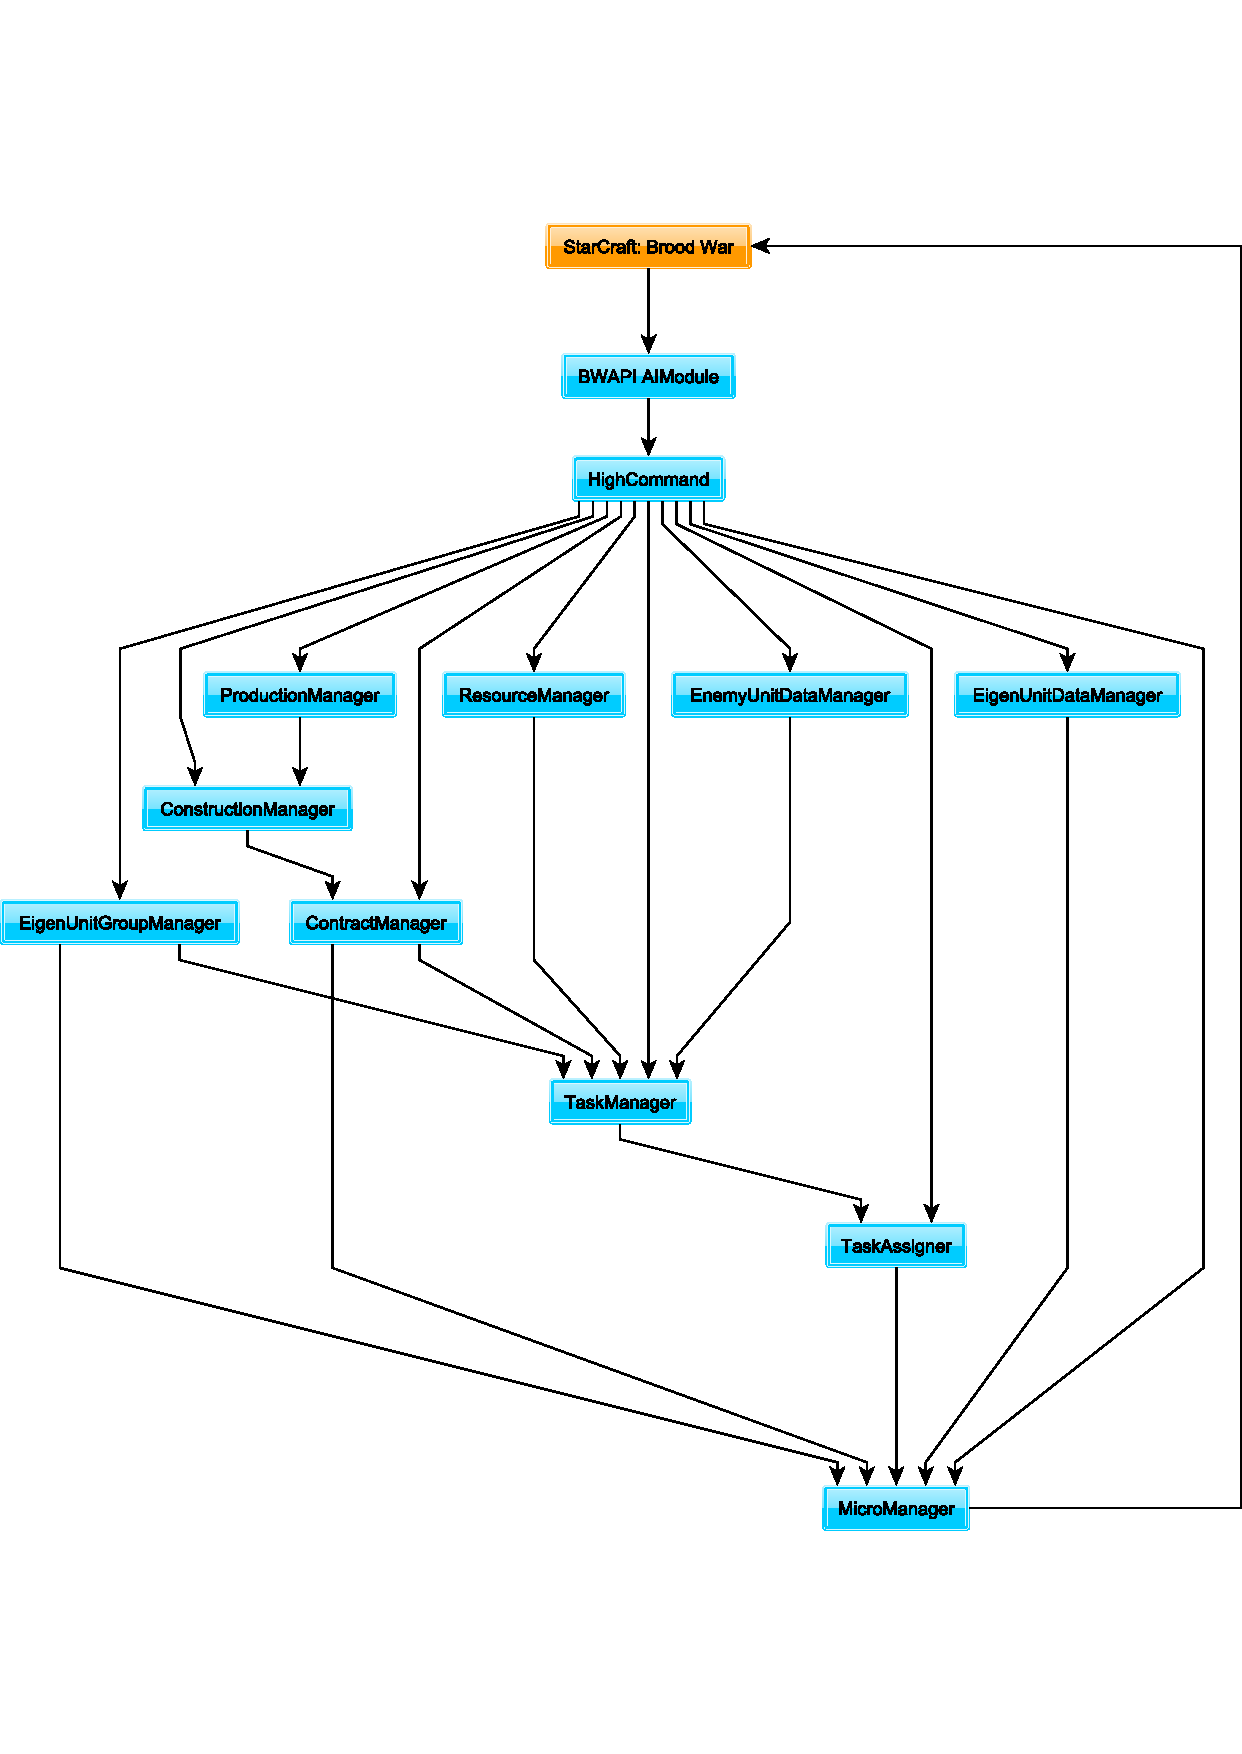
\includegraphics[width=\textwidth, trim= 0mm 30mm 0mm 30mm, clip]{images/flowofinformation}
\caption{The flow of information from StarCraft through Mass Expand to MicroManager, which sends commands back to StarCraft.}
\label{fig:flowofinformation}
\end{figure}

\section{HighCommand}

\section{EigenUnitDataManager}

\section{EigenUnitGroupManager}

\section{EnemyUnitDataManager}

\section{ResourceManager}

\section{TaskManager}

\section{TaskAssigner}

\section{ProductionManager}

\section{ConstructionManager}

\section{ContractManager}

\section{MicroManager}

\label{}